\documentclass[11pt,a4paper]{article}
\usepackage[utf8]{inputenc}
\usepackage[T1]{fontenc}
\usepackage{lmodern}
\usepackage{geometry}
\usepackage{booktabs}
\usepackage{amsmath}
\usepackage{graphicx}
\usepackage{float}
\usepackage{hyperref}
\geometry{margin=2.5cm}
\title{ASCAT Destekli TIGGE Rüzgar Tahminlerinde Thiessen Poligonları ve XGBoost ile Hata Düzeltmesi}
\author{İlayda}
\date{Pilot çalışma: Ocak 2021}
\begin{document}
\maketitle

\begin{abstract}
Bu çalışma, 12 saatlik TIGGE 10 m rüzgar tahminlerinin tahmin başlangıç zamanındaki ASCAT gözlemleri kullanılarak düzeltilmesini incelemektedir. ASCAT grid hücreleri, ASOS/LTB istasyonlarına Thiessen poligonlarıyla atanmış ve alan-ağırlıklı istasyon özellikleri XGBoost hata düzeltme modeline verilmiştir. Değerlendirme LTB/ASOS gözlemleri ve ERA5 reanalysis hedefleriyle, zaman sıralamasını koruyan beş katmanlı rolling-origin doğrulama kullanılarak yapılmıştır. Ocak 2021 pilot döneminde RMSE iyileşmesi sırasıyla yüzde 52.07 ve yüzde 50.04 bulunmuştur. LTB hedefinde Diebold--Mariano testi anlamlı iken, ERA5 hedefindeki sonuç daha uzun dönemle doğrulanmalıdır.
\end{abstract}

\section{Veri ve yöntem}
TIGGE tahmini 12:00 başlangıç zamanında alınmış, ASCAT aynı başlangıç zamanında kullanılmış, ERA5 ve LTB doğrulaması 12 saat sonraki geçerlilik zamanında yapılmıştır. LTB rüzgar hızı knot biriminden m/s'ye dönüştürülmüştür. Eksik hız değerleri nedensel Kalman filtresiyle doldurulmuştur.

\subsection{Rüzgar hızı ve hata}
\begin{equation}
U = \sqrt{u_{10}^2+v_{10}^2}
\end{equation}
\begin{equation}
e_t = U_t^{ERA5}-U_t^{TIGGE}, \qquad
\widehat{U}_t^{corr}=U_t^{TIGGE}+\widehat{e}_t(X_t).
\end{equation}

\subsection{Thiessen ağırlığı}
Her ASCAT hücresi en yakın istasyonun Voronoi/Thiessen hücresine atanmıştır. Enlem kaynaklı hücre alan farkı için $w_j=\cos(\phi_j)$ kullanılmıştır:
\begin{equation}
\overline{U}_{s,t}^{ASCAT} =
\frac{\sum_{j\in V_s}w_j U_{j,t}^{ASCAT}}
{\sum_{j\in V_s}w_j}.
\end{equation}

\subsection{Model ve doğrulama}
Ham TIGGE, sabit bias düzeltmesi, lineer regresyon, Random Forest ve XGBoost karşılaştırılmıştır. Zaman sıralaması korunmuş, beş expanding/rolling test katmanı kullanılmıştır. Tahmin başlangıcı ile geçerlilik zamanı için $t_{init}\le t_{valid}$ koşulu kontrol edilmiştir.

\subsection{İstatistikler}
\begin{equation}
RMSE=\sqrt{\frac{1}{n}\sum_i(\widehat{U}_i-U_i)^2},\quad
MAE=\frac{1}{n}\sum_i|\widehat{U}_i-U_i|
\end{equation}
\begin{equation}
z_i=\frac{x_i-\bar{x}}{s_x}.
\end{equation}
RMSE farkları 2000 tekrarlı paired bootstrap ile yüzde 95 güven aralığında raporlanmış, tahmin hatalarının karesel farkları için lag-1 Newey--West varyanslı Diebold--Mariano testi uygulanmıştır.

\section{Sonuçlar}
\begin{table}[H]\centering
\caption{Rolling-origin doğrulama sonuçları.}\label{tab:metrics}
\begin{tabular}{llrrrr}
\toprule
Hedef & Model & MAE & RMSE & $R^2$ & Örnek\\
\midrule
LTB & TIGGE & 2.645 & 2.988 & -103.187 & 18\\
LTB & ASCAT+XGBoost & 1.247 & 1.432 & -16.343 & 18\\
ERA5 & TIGGE & 2.032 & 2.386 & -17.259 & 18\\
ERA5 & ASCAT+XGBoost & 0.978 & 1.192 & -3.290 & 18\\
\bottomrule
\end{tabular}
\end{table}

\begin{figure}[H]\centering
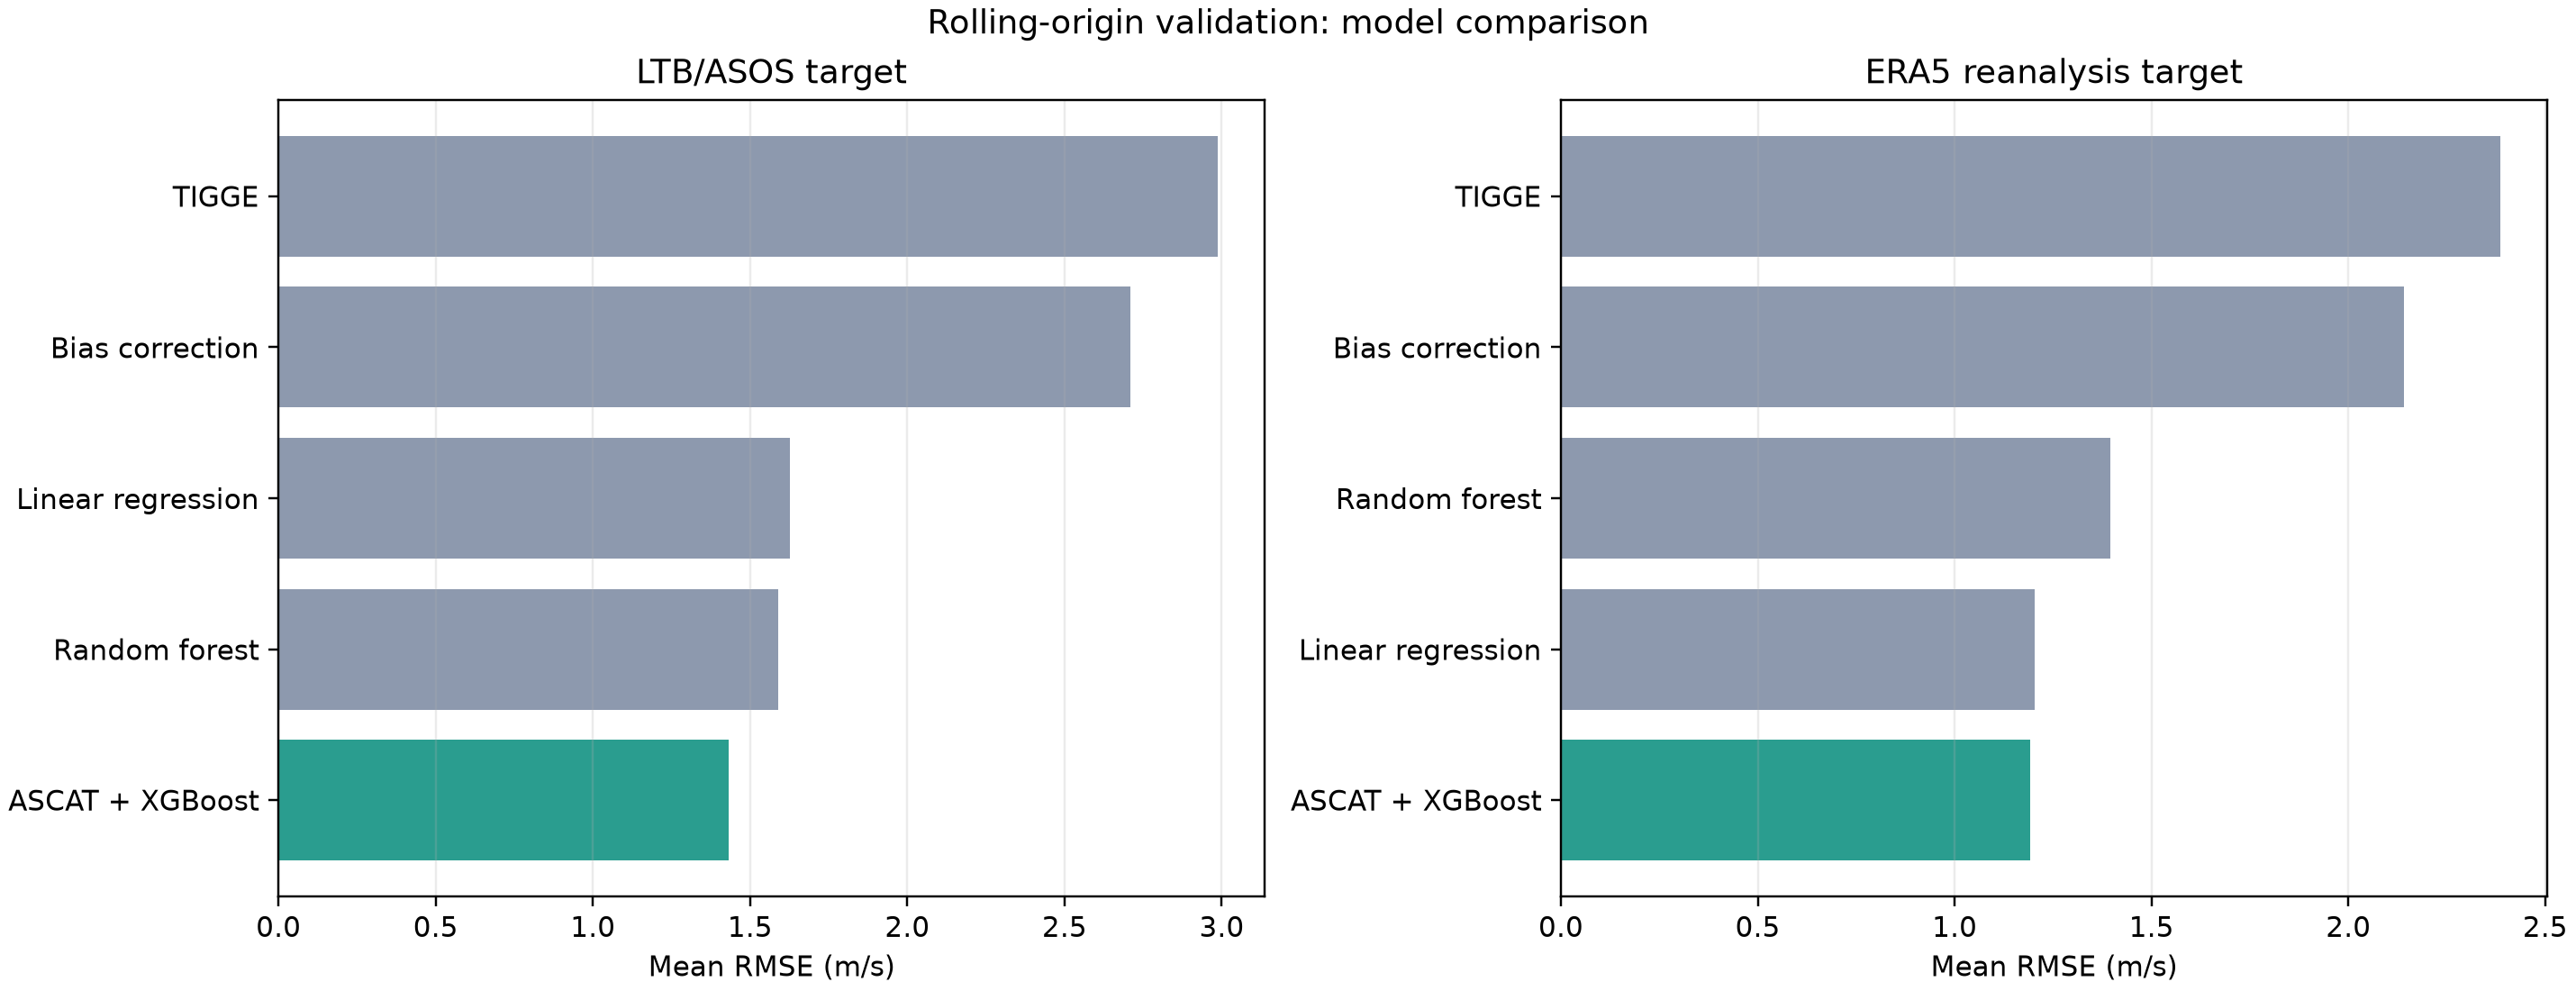
\includegraphics[width=.95\linewidth]{wind_correction_output/figures/model_rmse_comparison.png}
\caption{Model RMSE karşılaştırması.}\end{figure}
\begin{figure}[H]\centering
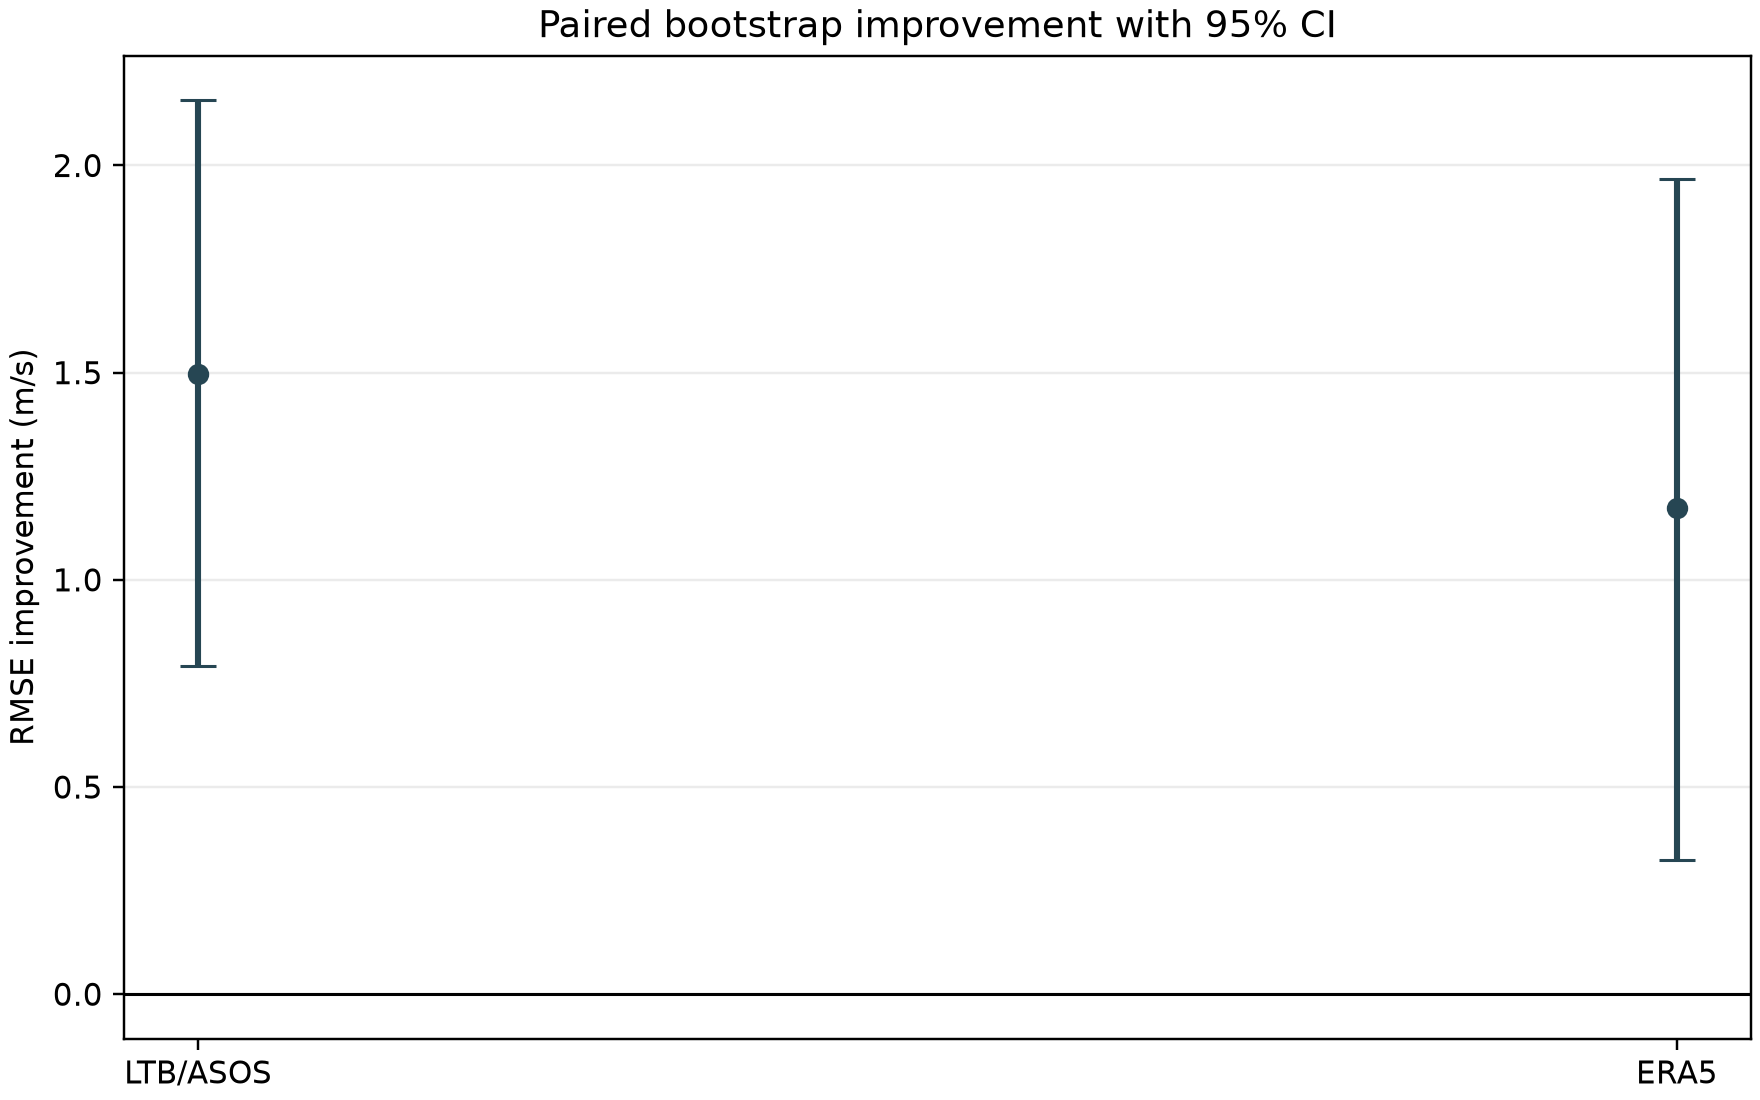
\includegraphics[width=.82\linewidth]{wind_correction_output/figures/rmse_bootstrap_improvement.png}
\caption{Paired bootstrap RMSE iyileşmesi ve yüzde 95 güven aralığı.}\end{figure}
\begin{figure}[H]\centering
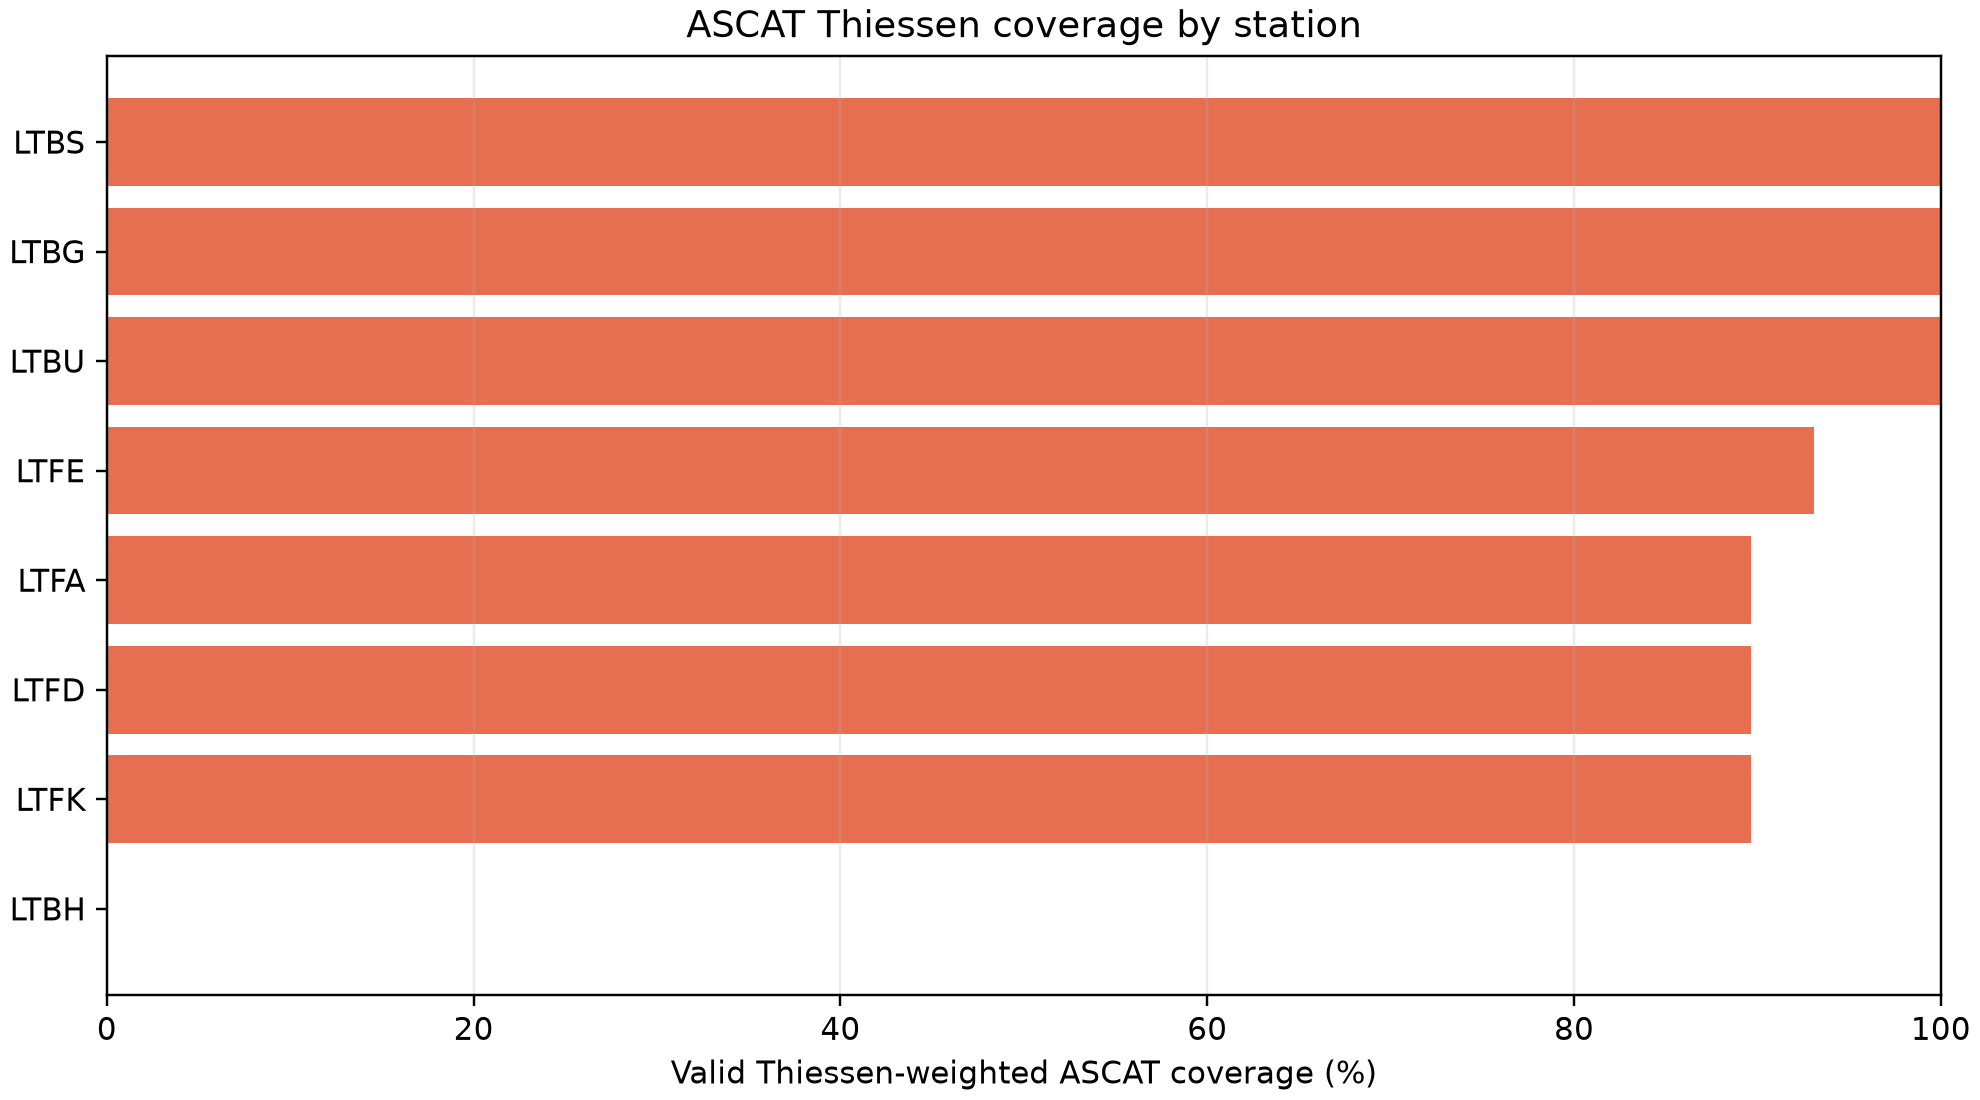
\includegraphics[width=.85\linewidth]{wind_correction_output/figures/thiessen_coverage.png}
\caption{Thiessen-ağırlıklı ASCAT geçerli veri kapsamı.}\end{figure}

\section{Kullanıcı görselleri}
Bu beş alan daha sonra bölge haritası, istasyon dağılımı, rüzgar profili, hata haritası ve zaman serisi görselleriyle doldurulabilir.
\begin{figure}[H]\centering\framebox{\parbox{.9\linewidth}{\vspace{3cm}\centering Kullanıcı Görseli 1 için yer\vspace{3cm}}}\caption{Kullanıcı görseli 1.}\end{figure}
\begin{figure}[H]\centering\framebox{\parbox{.9\linewidth}{\vspace{3cm}\centering Kullanıcı Görseli 2 için yer\vspace{3cm}}}\caption{Kullanıcı görseli 2.}\end{figure}
\begin{figure}[H]\centering\framebox{\parbox{.9\linewidth}{\vspace{3cm}\centering Kullanıcı Görseli 3 için yer\vspace{3cm}}}\caption{Kullanıcı görseli 3.}\end{figure}
\begin{figure}[H]\centering\framebox{\parbox{.9\linewidth}{\vspace{3cm}\centering Kullanıcı Görseli 4 için yer\vspace{3cm}}}\caption{Kullanıcı görseli 4.}\end{figure}
\begin{figure}[H]\centering\framebox{\parbox{.9\linewidth}{\vspace{3cm}\centering Kullanıcı Görseli 5 için yer\vspace{3cm}}}\caption{Kullanıcı görseli 5.}\end{figure}

\section{Sınırlılıklar}
Bu sonuçlar Ocak 2021 döneminde 18 bağımsız test örneğine dayanan pilot bulgulardır. LTB hedefinde DM testi $p=0.0077$, ERA5 hedefinde $p=0.0875$ bulunmuştur. ERA5 sonucu klasik yüzde 5 seviyesinde anlamlı değildir. Mevsimsel ve yıllararası genelleme için daha uzun TIGGE dönemleri gereklidir. LTBH istasyonunda geçerli Thiessen ASCAT değeri bulunmadığı için bu istasyon model tablosuna dahil edilmemiştir.
\end{document}
